\section{Materials preparation}

  \subsection{Cell lines}

    Transfection was always performed by lipofection~\Srefp{methods:lipofection},
    both for transient and stable cell lines. For creation of stable cell lines,
    cells were trypsinized and split 1:20 on \SI{10}{\cm} dishes 24~hours after transfection.
    After another 24 hours, Blasticidin-S was added to the medium for
    a final concentration of \SI{3}{\ug\per\ml} as found by performing a
    Blasticidin-S kill-curve \Srefp{sec:methods:kill-curve}.
    Cell growth was followed and medium replaced when appropriate.
    As cell colonies started to be visible by the naked eye, approximately
    3~weeks after plating, these were screened by fluorescence microscopy.
    Positive colonies were aspirated and moved into 24-well plates with
    \SI{1}{\ml} disposable pipette tips, and the thinnest extremity removed.

    \begin{figure}
      \centering
      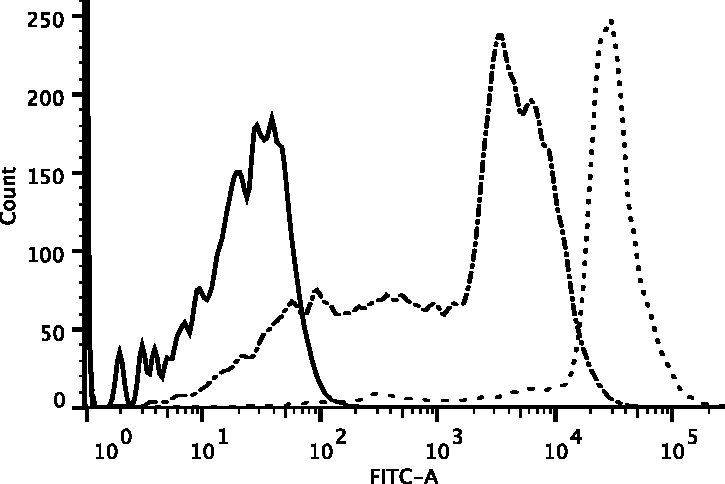
\includegraphics[width=\textwidth]{figs/facs-stable-cell-lines.pdf}
      \captionIntro{FACS sorting of mixed populations}
        {
          The multiple populations with differing intensity values were
          sorted by FACS. The full line represents the intensity profile
          of HeLa wild type cells; the dash-dot line, a mixed population
          of HeLa cells expressing H2B--EGFP; and the dotted line, the
          sorted population.
        }
      \label{fig:methods:facs}
    \end{figure}

    Populations with mixed levels of fluorescent intensity were frequently
    obtained while preparing stable cell lines. In such cases, cells with
    similar intensity of their corresponding fluorophore were FACS
    sorted \frefp{fig:methods:facs}.

    The following stable lines were prepared:

    \begin{itemize}
      \item HeLa H2B--EGFP
      \item HeLa H2B--EGFP D25G V118I
      \item HeLa H3--EYFP
      \item HeLa H3--EYFP T45A
      \item HeLa H3--EYFP T45E
      \item HeLa H4--EYFP
      \item HeLa H4--EYFP R45H
    \end{itemize}

  \subsection{Microscopy}

    Both stable and transiently cell lines were used in imaging as described.
    Transfection was performed 48~hours before imaging for transiently
    expressing cells.

    Confocal microscopy was performed with a Zeiss LSM510 Meta microscope
    using glass bottom LabTek II chambers. Wide-field fluorescence microscopy
    was performed with an Applied Precision DeltaVision Core system
    using \SI{35}{\mm} glass bottom MatTek dishes.

    In both cases, imaging was performed within an acrylic environmental
    chamber that fully enclosed the stage plate and microscope objectives.
    Temperature and CO$_2$ levels were maintained via separate units connected
    to the environmental chamber.

  \subsection{Computational analysis}

    Software used for image analysis and visualization was described in
    \Sref{sec:software:octave-frap}.
    Original source code written in Matlab for a previously
    reported circle FRAP model \citep{mcnally-frap-code} was kindly offered
    to us under the GNU General Public License (GPL) version~3 by the
    original authors. A port of this code for the GNU Octave language was
    prepared and made available under the same license.
